\section{Ocenianie wykonawców}

Ocenianie wykonawców to dość prosta funkcjonalność, którą posiadają klienci. Składa się na nią jeden ekran przedstawiony na rysunku \ref{fig:rate}. Ocena dokonywana jest poprzez zaznaczenie odpowiedniej liczby gwiazdek oraz wpisane opcjonalnego komentarza. Można dokonać jej tylko raz dla każdej oferty, bez możliwości późniejszej edycji.

Szczególnie zastanawiano się nad wyborem odpowiedniej metody, za pomocą której klienci mają wyrażać poziom swojej satysfakcji. Pomocny przy tym zagadnieniu okazał się artykuł Roberta Westbrooka \cite{rating-scale}, który porównuje efektywność mierzenia satysfakcji za pomocą różnych skal. Szczególnie zachęca do wykorzystania skali DT (ang. Delighted - Terrible), która wprowadza bardziej równomierny rozkład dla oddawanych ocen niż inne. Zdecydowano się jednak wykorzystać gotowy już komponent paska gwiazdek, by uniknąć problemów z implementacją. Z tego powodu dodano jedynie wyświetlany nad nim napis odpowiadający aktualnej jego wartości w skali DT, na przykład: neutralnie, raczej satysfakcjonująco, zadowalająco, czy zachwycająco. Poprzez taki zabieg miano nadzieję wykorzystać część korzyści płynących ze skali DT, bez nadmiernego nakładu pracy. Nie jest to bowiem element kluczowy.

\begin{figure}[ht]
  \centering
    \fbox{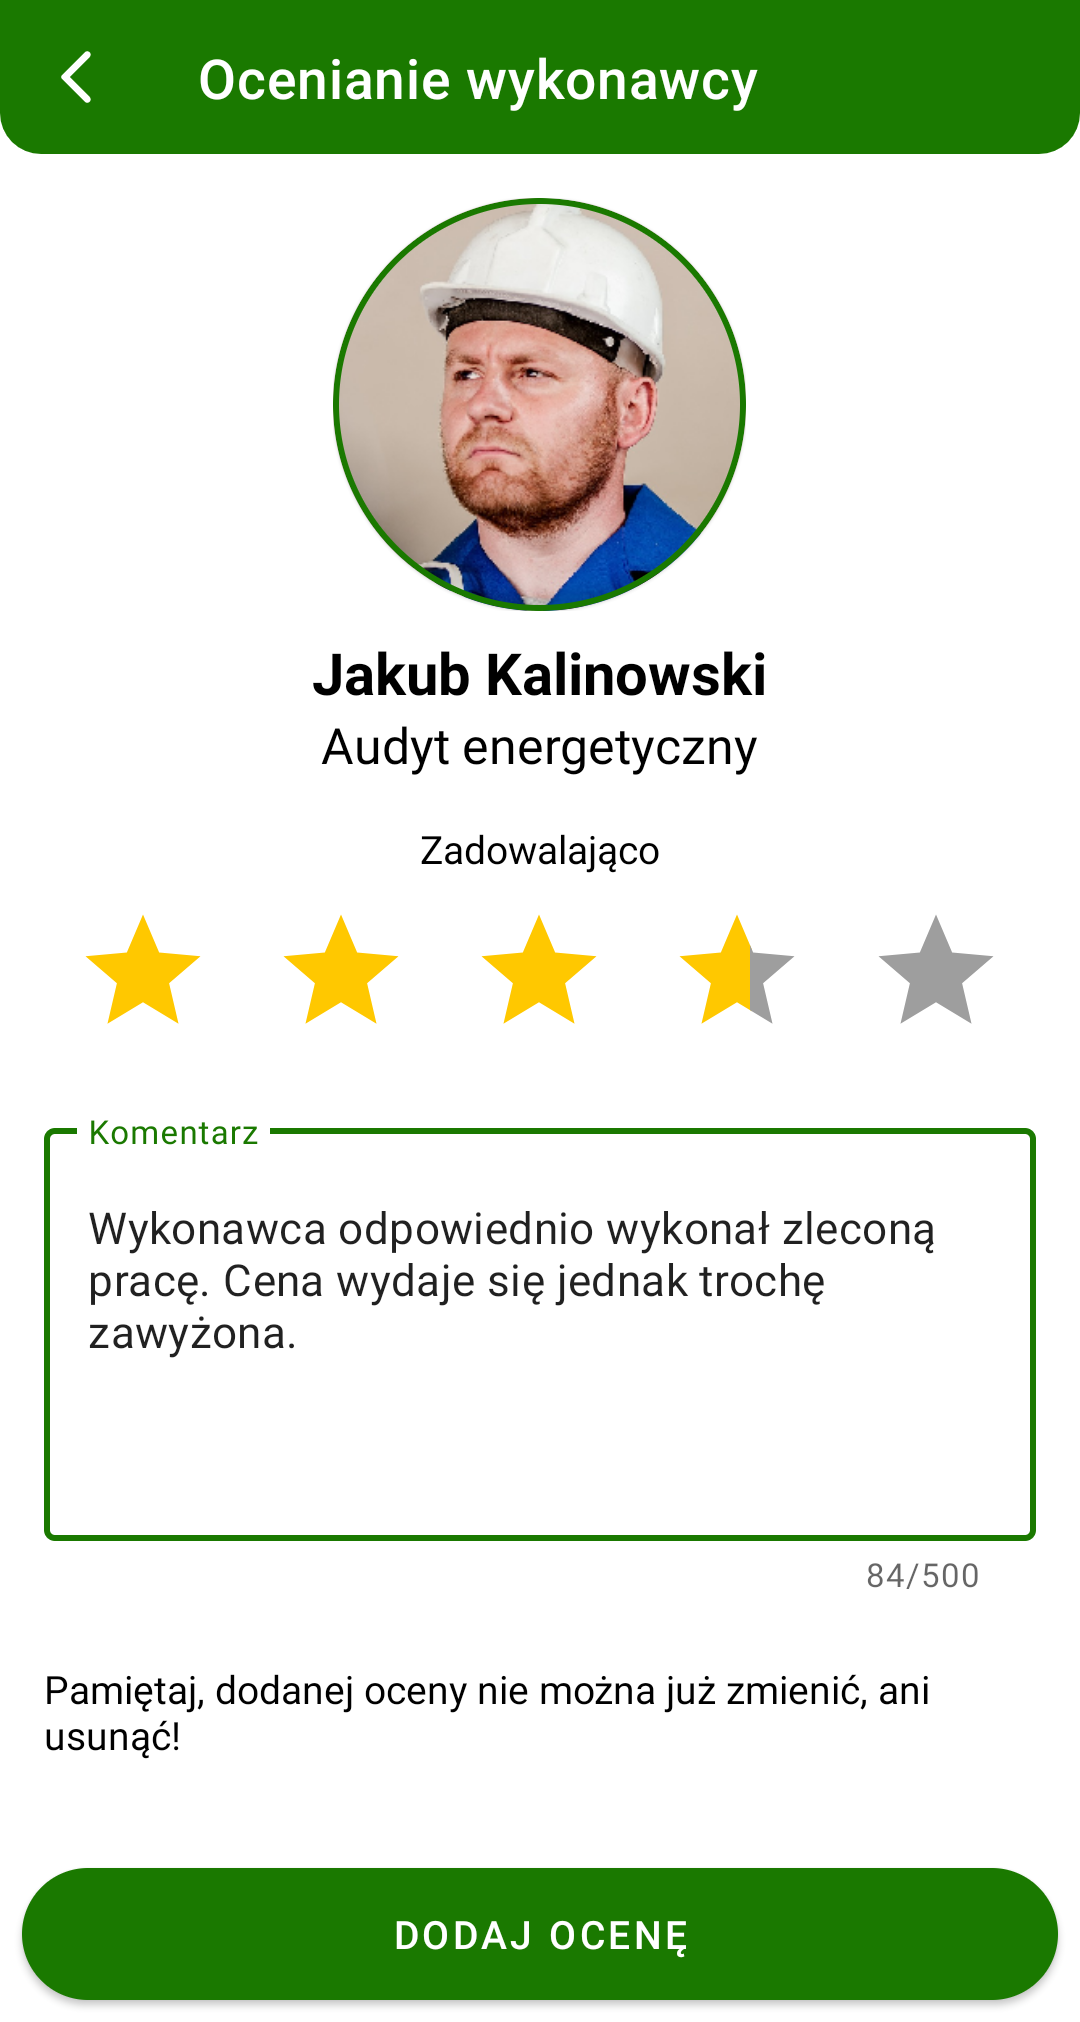
\includegraphics[width=0.33\linewidth]{screens/add_rating.png}}
  \caption{Ekran oceniania wykonawcy}
  \label{fig:rate}
\end{figure}

Wadą stworzonego systemu ocen, którą należy wskazać i zaznaczyć, jest to, że nie jest on do końca wiarygodny. Problem polega na tym, iż nieuczciwi wykonawcy mogą się zarejestrować również jako klienci, a następnie podjąć działania, których wynikiem będzie wystawienie samemu sobie pozytywnej oceny. Problem ten okazał się bardzo trudnym do rozwiązania. Najprostszym wyjściem jest zablokowanie możliwości oceniania, gdy konwersacja jest pusta lub zlecenie zostało dopiero utworzone. Są to jasne przesłanki co do próby oszustwa, lecz takie zabezpieczenie jest proste do obejścia. Bardziej rzetelną metodą byłaby konieczność walidacji wszystkich komentarzy przez moderatorów, którzy mieliby dostęp do konwersacji i pozostałych informacji. Mimo wszystko wciąż nie jest to rozwiązanie pewne, ponieważ informacje te mogły zostać w dobry sposób spreparowane. Z technicznego punktu widzenia dla moderatorów potrzebny byłby również kolejny interfejs, co wiążę się z dalszą komplikacją projektu. Z wymienionych przyczyn postanowiono zaakceptować brak pełnej wiarygodności ocen i zostawić rozwiązanie tego problemu na ewentualne dalsze etapy rozwoju projektu.